\section{Observations}

\begin{frame}{DDT}

  \begin{beamerboxesrounded}{DDT Properties}
    \begin{itemize}
      \item Highest value: 4 (Probability $\frac{4}{256}$)
      \item Only contains the values 0, 2 and 4
      \item For any fixed input/output difference
            \begin{itemize}
              \item 4 occurs exactly once
              \item 2 occurs 126 times
              \item 0 occurs 129 times
            \end{itemize}
      \item No of zeroes is 33,150. $\sim$ 50\% difference pairs are impossible.
    \end{itemize}
  \end{beamerboxesrounded}

  Very similar to AES Sbox

\end{frame}

\begin{frame}{Integral Attack}
  \begin{flalign*}
    P_0 &= (0, c_1, c_2 \dotsc c_{15})\\
    P_1 &= (1, c_1, c_2 \dotsc c_{15})\\
    P_2 &= (2, c_1, c_2 \dotsc c_{15})\\
    &\vdots\\
    P_{255} &= (255, c_1, c_2 \dotsc c_{15})
  \end{flalign*}

  \begin{equation*}
    \Lambda = \{P_0, P_1, P_2 \dotsc P_{255}\}
  \end{equation*}
\end{frame}

\begin{frame}{Integral Attack}{Properties}
  \begin{beamerboxesrounded}{All $\mathcal{A}$}
    The byte in which all values appear exactly once among all the
    texts in the set is called the \textbf{all} property.
  \end{beamerboxesrounded}

  \vspace{5mm}

  \begin{beamerboxesrounded}{Constant $\mathcal{C}$}
    The byte in which all texts in the set have an identical value is called the \textbf{constant} property.
  \end{beamerboxesrounded}

  \vspace{5mm}

  \begin{beamerboxesrounded}{Balanced $\mathcal{B}$}
    The byte in which XOR sum of all values is zero is called the \textbf{balanced} property.
  \end{beamerboxesrounded}
\end{frame}

\begin{frame}{Integral Attack}{Distinguisher}
  \begin{figure}
    \centering
    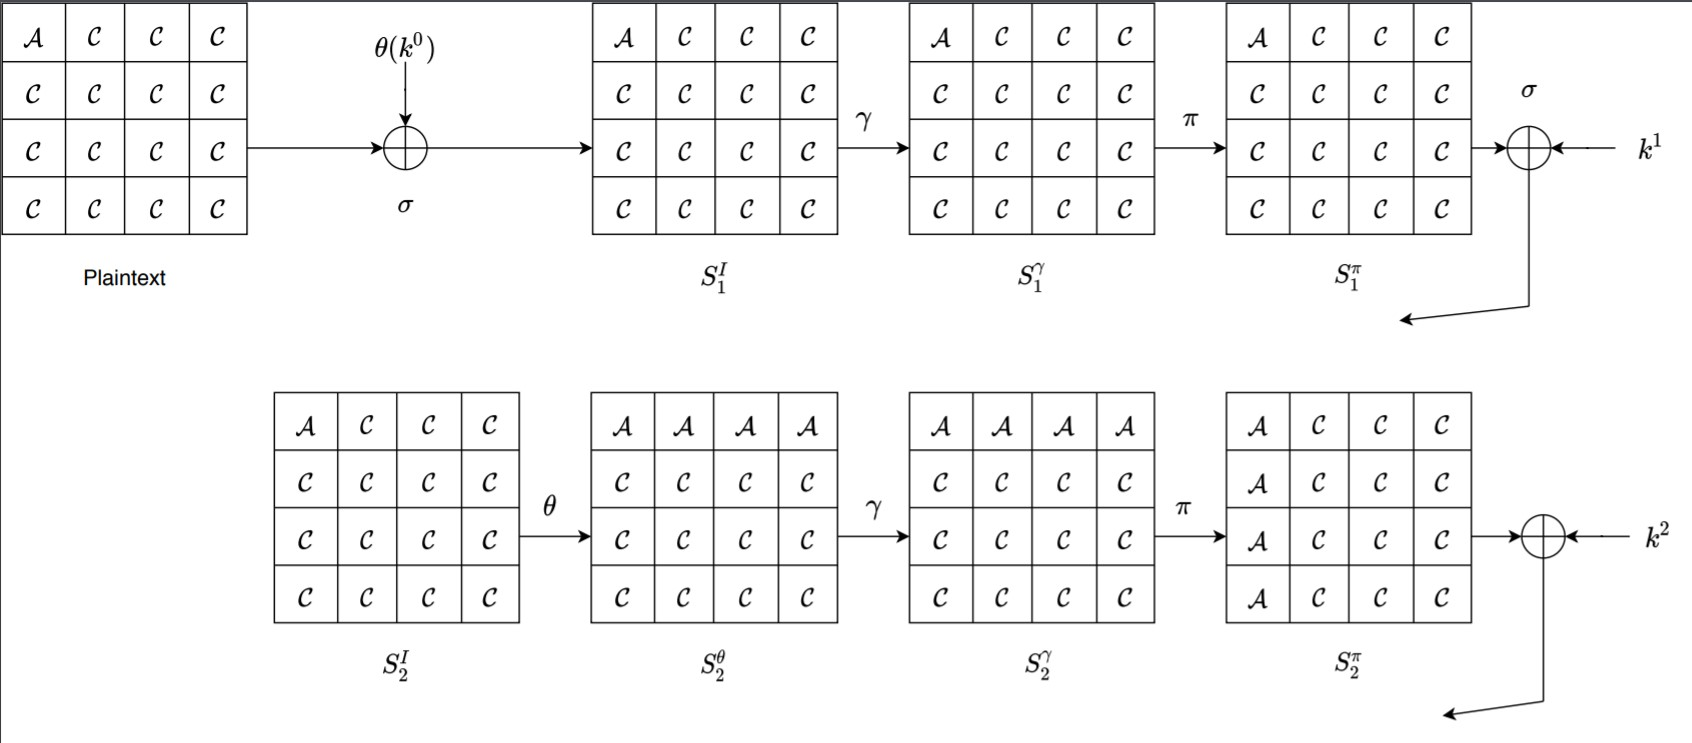
\includegraphics[width=\linewidth]{sq_attack1}
    \caption{Integral attack distinguisher (Round 1, 2)}
  \end{figure}
\end{frame}

\begin{frame}{Integral Attack}{Distinguisher}
  \begin{figure}
    \centering
    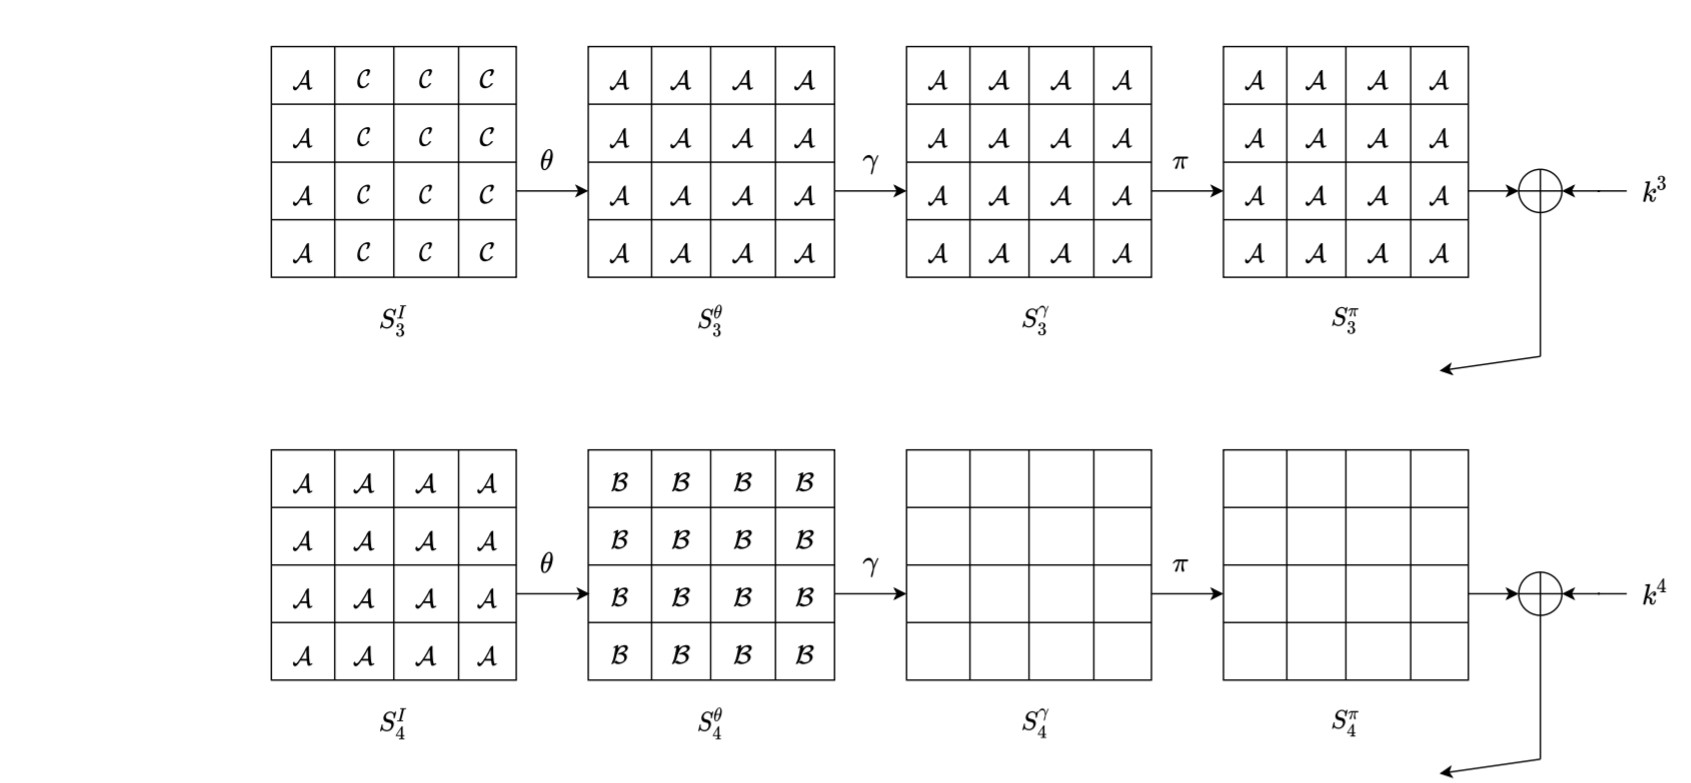
\includegraphics[width=\linewidth]{sq_attack2}
    \caption{Integral attack distinguisher (Round 3, 4)}
  \end{figure}
\end{frame}

\begin{frame}{Integral Attack}{Balanced Property}
  \begin{flalign*}
    \bigoplus_{0 \leq n \leq 255} S_{4,n}^\theta[i,j]
    &= \bigoplus_{0 \leq n \leq 255} \bigoplus_k c_{j-k} S_{4,n}^I[i,k] \label{eq:bal} \\
    &= \bigoplus_l c_l \bigoplus_{0 \leq n \leq 255} S_{4,n}^I[i,l+j] \nonumber \\
    &= \bigoplus_l c_l 0 \nonumber \\ &= 0 \nonumber
  \end{flalign*}
\end{frame}

\begin{frame}{Integral Attack}
  \begin{beamerboxesrounded}{Attack Procedure}
    \begin{itemize}
      \item Guess a byte from $k^4$, say $k^4_{i,j}$.
      \item Use the guess $k^4_{i,j}$ to calculate $S_4^\theta[j,i]$
            \begin{equation*}
              S_4^\theta[j,i] = Sbox^{-1}[S_5^I[i,j] \oplus k_{i,j}^4]
            \end{equation*}
      \item Verify the XOR sum of all 256 values of $S_4^\theta[j,i]$. If it is not balanced then wrong guess.
    \end{itemize}
  \end{beamerboxesrounded}
\end{frame}

\begin{frame}{Integral Attack}
  \begin{beamerboxesrounded}{Sets required}
    \begin{itemize}
      \item Probability that a random XOR sum of 8 bit is zero is $2^{-8}$
      \item With $2^8$ guesses, expected number of subkeys passing is $2^8.2^{-8} = 1$.
      \item Theoretically, 1 $\Lambda$ set is just enough.
      \item For practical purposes, 2 $\Lambda$ sets need to be used for high success probability.
    \end{itemize}
  \end{beamerboxesrounded}

  \vspace{5mm}

  \begin{beamerboxesrounded}{Extended Attacks}
    The 4 round attack can be extended from beginning and end. The $(D,T,M)$ complexities of the 6 round attack are $(2^{32},2^{72},2^{32})$.
  \end{beamerboxesrounded}
\end{frame}

\begin{frame}{Other Attacks}
  \begin{beamerboxesrounded}{Related Key Boomerang Attack}
    \begin{itemize}
      \item Attack on full 8 round cipher
      \item 7 round distinguisher with probability $2^{-119}$
      \item Retrieve 16 bits of key using $2^{123}$ data and $2^{36}$ time
    \end{itemize}
  \end{beamerboxesrounded}
  \vspace{5mm}
  \begin{beamerboxesrounded}{Biclique Cryptanalysis}
    \begin{itemize}
      \item Attack on full 8 round cipher inspired by Biclique Cryptanalysis of AES
      \item $(D,T,M)$ complexities are $(2^{48},2^{126},2^{16})$
    \end{itemize}
  \end{beamerboxesrounded}
\end{frame}